\chapter{Implementation}

\section{Technologies Used}

\subsection{Datasets}
In the process of conducting this experiment, there are two types of datasets. 
The set of fist image datasets are from kaggle.com. The datasets is made up of two classes, those that are with masks and the others that are without masks.
That is a total of 1412 images belonging to 2 classes in training set and 290 images in testing set.


    \centerline{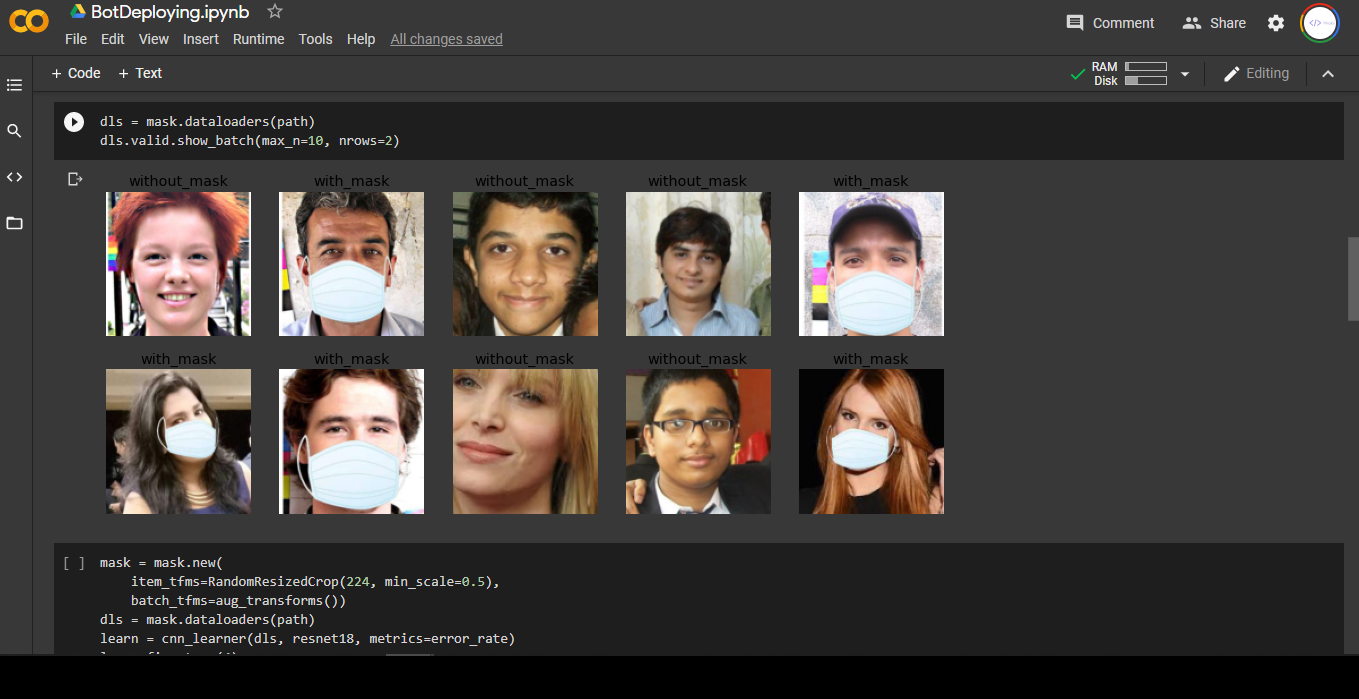
\includegraphics[width=.6\textwidth,height=.5\textheight,keepaspectratio]{tex/images/Screenshot_Masks.png}}
     \caption{Screenshot from my Google Colab}
    \label{fig}

This is what the dataset looks like. We have pictures of people wearing masks and others not wearing masks.  This dataset provides a great variation of faces
this making this dataset useful. To my knowledge this dataset is one of the largest datasets that was released on kaggle that has faces of masks and no masks and made available thanks to Prajna Bhandary.
This dataset was a collection of random faces of people and with the aid of photoshop, some faces were then added masks to make them fit on the face\vspace{5mm}. 

The second set of images are my own collection, where I personally asked people that I know to send me pictures of themselves
with masks, others without so that I can compile a dataset made up of real-world masked faces and capture the different mask colors and shades. The dataset of faces where people were wearing masks since were mostly edited contained a lot of noise and some even had repetitions in the datasets. Since we need our model to produce an accurate prediction when trained, all the above mentioned had to be handled with caution. The dataset was then processed and repetitions were removed manually by myself. I further performed the data cleaning manually to remove the found images. Due to human error, it is possible that there exist some images that still fall under the above mentioned since the process was a long and tiresome one.  
\subsection{Convolutional Neural Network}
As mentioned above how useful Convolutional neural networks are when it comes to classification of images and videos we have classified our images using InceptionV3. InceptionV3 is a Deep Neural Network that is used for classification problem, much like MobileNetV2 but much more powerful.What makes InceptionV3 stand out is that it is a transfer learning pre-trained model that is a 48 layered convolutional neural network. Further explanation is given in the next subsection.
\vspace{5mm}.

Network architecture of InceptionV3:
InceptionV3 is the model that was used for our system. It contains three kinds of Inception modules, Inception A, Inception B and Inception C. These inceptions are well-designed convolutional modules that are able to generate both discriminatory features and be of paramount assistance in reducing number of parameters. One Inception module consists of a number of convolutional layers as well as pooling layers in parallel. Smaller convolutional layers such as 3x3,1x3,3x1 and 1x1 layers, are useful in in the Inception modules to help reduce the number of parameters. In Inception-v3, 3 Inception A modules, 5 Inception B modules and 2 Inception C modules are stacked in series.\cite{guan2019deep}.
\vspace{5mm}

Below is the Convolutional Layer of InceptionV3:

\vspace{3}.
\begin{tabular}{ |p{3cm}||p{3cm}|p{3cm}|p{3cm}|}
    \hline
    \multicolumn{3}{|c|}{InceptionV3 Network} \\
    \hline
     Layer & Patch Size & Input Size\\
    \hline 
    conv & 3x3/2 & 150x150x3\\
    \hline
    conv & 3x3/1 & 255x255x32\\
    \hline
    conv padded & 3x3/1 & 255x255x32\\
    \hline
    pool & 3x3/2 & 7x7x64\\
    \hline
    conv & 3×3/1 & 73×73×64\\
    \hline
    conv & 3×3/2 & 71×71×80\\
    \hline
    conv & 3×3/1 & 35×35×192\\
    \hline
    3×Inception & - & 35×35×288\\
    \hline
    5×Inception & - & 17×17×768\\
    \hline
    2×Inception & - & 8×8×1280\\
    \hline
     pool & 8 × 8 & 8 × 8 × 2048\\
    \hline 
    linear & logits & 1 × 1 × 2048\\
    \hline
    softmax & classifier & 1 × 1 × 1000\\
    \hline
\end{tabular}
\vspace{5mm}

The implementation on our IDE looks like the code below based on the table presented above
\begin{lstlisting}
pre_trained_model = InceptionV3(include_top=False, weights='imagenet', input_shape=(150, 150, 3))

pre_trained_model.summary()

for layer in pre_trained_model.layers:
    layer.trainable = False

last_layer = pre_trained_model.get_layer('mixed7')
print('Last layer output shape :', last_layer.output_shape)
last_output = last_layer.output

x = tf.keras.layers.Flatten()(last_output)
x = tf.keras.layers.Dense(1024, activation='relu')(x)
x = tf.keras.layers.Dropout(0.3)(x)
#The Final layer with 3 outputs for 3 categories
x = tf.keras.layers.Dense(2, activation='softmax')(x)
model = tf.keras.models.Model(inputs=pre_trained_model.input, outputs=x)
model.summary()

model.compile(optimizer='adam', loss='binary_crossentropy', metrics=['accuracy'])
\end{lstlisting}

The above code shows the introduction of InceptionV3 and its parameters like how we explained above. We used input shape 150x150x3. In the final layer we have three outputs for three categories. We also compile using 'adam' as our optimizer.
\vspace{4mm}

In the earlier model that was used when we were training using MobileNets we used a code that looks like the one below:

\begin{lstlisting}
model = Sequential([
    Conv2D(100, (3, 3), activation='relu', input_shape=(150, 150, 3)),
    MaxPooling2D(2, 2),

    Conv2D(100, (3, 3), activation='relu'),
    MaxPooling2D(2, 2),

    Flatten(),
    Dropout(0.9),
    Dense(63, activation='relu'),
    Dense(2, activation='softmax')
])

\end{lstlisting}
\vspace{4mm}

The above code shows a bit more detailed how the model is constructed and what parameters are inside a convolution. As it can be seen, we have Conv2D, MaxPooling2D as our layers, followed by a Flatten used to flatten out the images after extraction, dropout to do some cleaning and finishing them off with Dense layers.

\subsection{Transfer Learning and Pre-Training}
In the process of Transfer learning, we used the approach were all convolutional neural network layers excluding the last one are fine-tuned at learning rate that is smaller than the normal learning rate. The last layer is fine-tuned and freshly trained to suite the current  problem at hand. The last layers that we introduced are an average pooling layer with a pool size of 2.It consists of 3 outputs for the purpose of 3 categories.It has a dense layer consisting of 1024 neurons with Relu activation function and a dropout rate of 0.3, and finally a dense layer with two neurons and a softmax activation function is added to make classification. Transfer Learning model is trained for 100 epochs with each epoch having a callback that takes in a checkpoint as an index.
The code is similar to the one included above when it comes to the Final Layers that we used to fine-tune our classification problem to obtain accurate results.

\begin{lstlisting}
pre_trained_model = InceptionV3(include_top=False, weights='imagenet', input_shape=(150, 150, 3))

pre_trained_model.summary()
\end{lstlisting}
\vspace{4mm}

A code for the pre-trained model and its summary is given by the code above.This model initialized above is enough to give a complete summary of the model. It is important to note that this piece of code is much more complex than this line that we see here. It is actually a complete Algorithm that has been fully trained before and was compiled to be in this way to help with this paradigm og transfer learning. The last layers have been removed and we have added our own to fit the current system that we are working on. The code included in the subsection above gives a full description of that. It is also important to note that in our pre-trained model we have specified the input shape. there is an option to leave that out. The default input shape of InceptionV3 is 299x299x3, how ever, we used 150x150x3. We also had an option to include and specify the average pooling output but we decided to leave that out as well. We used weights 'mangenet' another option we had was to make it a random weight by equating it to None to look like this \begin{lstlisting}
weights = None
\end{lstlisting}
We also had the option to include our input tensor but we decided to leave that one out also. Running the code above will load the model, download the weights since it is required, and finally will give a summary of the model architecture which will serve as a confirmation that it loaded correctly.
   
\subsection{Training}
The training is an involvement of retraining the model with the dataset. Using the directory to get the training set and using a method called ImageDataGenerator.
After the model has been trained. the model summary is prented and then compile the model using an optimizer adam, loss of categorical crossentropyand metrics of accuracy.The training generator:
\begin{itemize}
    \item rescale = 1.0/255
    \item rotation range=40
    \item widt shift range=0.2
    \item height shift range=0.2
    \item shear range=0.2
    \item zoom range=0.2
    \item horizontal flip=True
    \item fill mode='nearest
\end{itemize}

Furthermore, the batch size is 10 and target size is set to 150, 150.

Previously, the model used was MobileNets. MobileNets is built on a simplified architecture that utilizes deeply separable convolutions to create the CNN. \cite{alsing2018mobile}.

The code for training looks like this:
\begin{lstlisting}
TRAINING_DIR = "C:/Users/silab/Desktop/MaskDetectionThesis/Datasets/observations/experiements/dest_folder/train"
train_datagen = ImageDataGenerator(rescale=1.0/255,
                                   rotation_range=40,
                                   width_shift_range=0.2,
                                   height_shift_range=0.2,
                                   shear_range=0.2,
                                   zoom_range=0.2,
                                   horizontal_flip=True,
                                   fill_mode='nearest')

train_generator = train_datagen.flow_from_directory(TRAINING_DIR,
                                                    batch_size=10,
                                                    target_size=(150, 150))
\end{lstlisting}    
\vspace{4mm}

What is notable from the training code above is that we have a Training directory that navigates to the directory of the dataset in the system since we are using Pycharm and everything is done on the local system. Training data-generator uses ImageDataGenerator as explained above. We then have to generate our training data-generator by adding the batch size and target size.
\vspace{5mm}
Training a model goes hand-in hand with Testing as well as Validation, The implementation is almost the same, however they are all equally important since the dataset is divided and images used to train, the ones used to test and the ones used to validate are all different. The validation code is given below:
\vspace{5mm}
\begin{lstlisting}
VALIDATION_DIR = "C:/Users/silab/Desktop/MaskDetectionThesis/Datasets/observations/experiements/dest_folder/val"

validation_datagen = ImageDataGenerator(rescale=1.0/255)
validation_generator = validation_datagen.flow_from_directory(VALIDATION_DIR,
                        batch_size=10,
                        target_size=(150, 150))
\end{lstlisting}
\vspace{4mm}
The validation, like training, also has its own directory to the dataset that deals with it, followed by the validation data-generator, which is then followed by the generator including the batch size and target size.
\subsection{Variational Autoencoder}
\subsection{Tensorflow}
\subsection{OpenCV}